\section{Results}
\label{sec:results}

\subsection{Validation context and disjoint endpoints}
\label{sec:current_detector_results}

The operating threshold was calibrated on 20,002 catalogue-negative examples
before endpoint scoring. At \(t_{10^{-3}}=1.572\), 20 calibration examples
met or exceeded threshold; Appendix~\ref{app:technical_validation} gives the
full-precision float32 value and comparison rule.

In the separate achieved-FPR endpoint, 13 of 12,512 catalogue-negative rows
exceed \(t_{10^{-3}}\), or 0.104 per cent. The row-Wilson 95 per cent
interval is [0.061, 0.178] per cent, and the spatial-group multiplier
interval is [0.055, 0.166] per cent. This is the threshold-exceedance rate for
the fixed evaluation cohort at the previously calibrated operating point.

The detector also responds to 39 of the 43 selected confirmed systems
(90.7 per cent). We report this selected-cohort fraction without a population
interval because the systems combine heterogeneous discovery programmes,
catalogue eligibility, and galaxy- and cluster-scale lenses.
Section~\ref{sec:checkpoint_sensitivity_results} reports this endpoint for the
12 sensitivity checkpoints. Appendix~\ref{app:technical_validation} reports
the separate noisy-label development diagnostics; threshold calibration and
selected-system evaluation use the cohorts defined above.

\subsection{\(G_{\rm domain}\) linear-probe separation}
\label{sec:domain_probe_results}

Observed references and simulated injections are distinguishable in all four
feature protocols (Table~\ref{tab:gdomain_four_rep}). Cross-fitted
domain-ranking AUC is 0.991 in the
operational detector's pooled penultimate representation, 0.958 in Stein
self-supervised survey features, 0.979 in generic ImageNet features, and
0.981 in pixel statistics. Thus strong separation appears in the lens-trained
representation, external learned representations, and elementary image
summaries.

\begin{table*}
\caption{Domain-ranking AUC on the same 43 observed and 6,336 injected rows.
The first four rows are cross-fitted domain probes. ``Fold range'' gives their
minimum and maximum fold AUC; folds contain only 8 or 9 observed systems. The
fixed operational lens head is a non-cross-fitted baseline on the same roster
and weights.}
\label{tab:gdomain_four_rep}
\centering
\begin{tabular}{lrrrl}
\toprule
Readout & Dimension & Domain-ranking AUC & Fold range & Evaluation \\
\midrule
Operational penultimate & 1\,280 & 0.991340 & 0.985--0.999 &
Cross-fitted domain probe \\
Stein SSL & 2\,048 & 0.958187 & 0.929--1.000 &
Cross-fitted domain probe \\
Generic ImageNet & 1\,280 & 0.978528 & 0.953--0.994 &
Cross-fitted domain probe \\
Pixel statistics & 18 & 0.980745 & 0.938--0.997 &
Cross-fitted domain probe \\
\midrule
Fixed operational lens head & -- & 0.980306 & -- &
Not cross-fitted \\
\bottomrule
\end{tabular}
\end{table*}

The existing lens-classification head also separates these populations
strongly (Table~\ref{tab:gdomain_four_rep}), showing that the difference is
expressed in the operational score as well as the fitted penultimate readouts.
The two readouts share a feature vector; no significance test compares their
AUCs. Each finite-cohort AUC describes its feature protocol, including its
training history, preprocessing, and fitted readout. Native-score summaries appear in
Appendix~\ref{app:four_representation_diagnostics}.

\subsection{\(G_{\rm match}\) shared-axis diagnostics}
\label{sec:matched_probe_results}

The score-blind \(G_{\rm match}\) design contains 43 triplets: each selected
observed reference, one matched bare \(G_{\rm rec}\) target, and that target with
its fixed 1.5-arcsec injection. The cross-fitted axis in each representation
is learned from observed-reference and bare-target rows only; injected rows are
not used to fit the axis or its scale. There are 129 rows in 43 dependency
components. Appendix Table~\ref{tab:gmatch_coverage} reports the measured
reference, complete-target-roster, and matched-target covariate ranges.

Mean injected-minus-bare movement along the operational observed--bare axis is
\(+0.023\), with median \(+0.0175\), in training-bare standardized-score
units. Twenty-seven targets move toward the observed-positive side and 16 in the
opposite direction; individual movements range from \(-0.453\) to \(+0.998\).
The mean signed movement is therefore near zero despite heterogeneous
pairwise shifts. The pooled injected-versus-bare AUC on this axis is 0.509.
Unlike \(G_{\rm domain}\), this analysis asks how adding a fixed source moves
the same target along an axis fitted between observed systems and bare
targets. Mean movements in Stein,
ImageNet, and pixel features are \(+0.235\), \(+0.025\), and \(-0.029\),
respectively. The Stein movement distribution is asymmetric: its median is
\(-0.069\), 12 movements are positive and 31 negative, and the range is
\(-0.982\) to \(+5.204\). It therefore does not indicate that most matched
targets move toward the observed side. Table~\ref{tab:gmatch_final} reports
the corresponding pooled AUCs.

Among 18 statistics, the \(z\)-band median has univariate AUC 0.888, and
omitting it lowers multivariate pixel AUC from 0.981 to 0.932 in
\(G_{\rm domain}\). Separately, within the 43 \(G_{\rm match}\) triplets, its
unweighted finite-cohort mean is 0.011448 in observed references, 0.005088 in
bare targets, and 0.005094 after injection. This matched bare--injected
comparison shows that the leading observed--injected offset is already present
before source insertion. This pixel-level result does not establish which
features drive the operational detector.

\begin{table*}
\caption{\(G_{\rm match}\) shared-axis pooled OOF AUC diagnostics for the 43
triplets. The axis is fitted on observed and bare rows; all entries are
finite-cohort point estimates without formal intervals.}
\label{tab:gmatch_final}
\centering
\small
\setlength{\tabcolsep}{4pt}
\begin{tabular}{lrrr}
\toprule
Representation & Obs.--bare & Obs.--inj. & Inj.--bare \\
\midrule
Operational penultimate & 0.998 & 0.998 & 0.509 \\
Stein SSL & 0.979 & 0.982 & 0.488 \\
ImageNet & 0.973 & 0.971 & 0.500 \\
Pixel statistics & 0.928 & 0.933 & 0.478 \\
\bottomrule
\end{tabular}
\end{table*}

\subsection{Conditional recovery and fixed-target brightness response}
\label{sec:recovery_results}

Conditional \(G_{\rm rec}\) recovery is 3.45 per cent (95 per cent
spatial-group interval, 3.10--3.83 per cent) under equal weighting of
observing cells, injection targets, and Einstein radii. This is 1,710
detections among 49,500 scenes generated from 4,500 targets in 2,187 spatial
groups. Two bare
targets exceed the same threshold. Across target--radius comparisons, 22 are
positive both before and after injection, 1,688 become positive, none becomes
negative, and 47,790 remain negative. The injection therefore raises the
positive-call rate by 3.41 percentage points across the specified grid.

The grid applies no rendered-arc visibility or S/N admission rule; its
estimand therefore averages all designed scenes rather than a visibility-selected
subset. Scene-weighted recovery is 8.45, 1.90, and 0.12 per cent in intrinsic source-magnitude bins
\([23,24)\), \([24,25)\), and \([25,26)\), respectively
(Table~\ref{tab:grec_brightness}). The final design also contains 99
cell--radius estimates: 500 targets at each radius in each of nine occupied
PSF--depth cells. Appendix~\ref{app:cell_radius_response} reports that
conditional response surface and its one empty PSF--depth combination.

Figure~\ref{fig:grouped_recovery} shows the equal-cell, equal-target response by
Einstein radius. Recovery is 0.044 per cent at 0.5 arcsec, reaches 6.22 per
cent at 2.5 arcsec, and is 6.02 and 5.47 per cent at 2.75 and 3.0 arcsec.
The simultaneous 95 per cent band has half-width 0.82 percentage points.

\medskip
\begin{center}
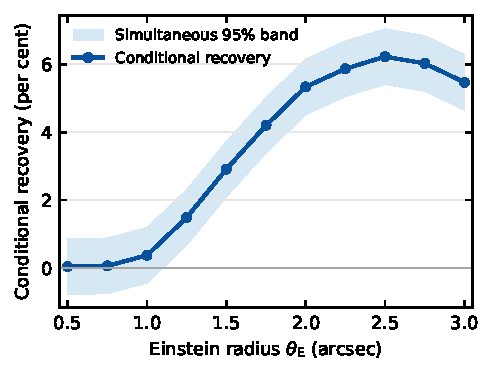
\includegraphics[width=\columnwidth]{figures/section5_grouped_recovery.pdf}
\end{center}
\refstepcounter{figure}\label{fig:grouped_recovery}
\noindent\textbf{Figure~\thefigure.} Conditional \(G_{\rm rec}\) recovery at the
\(t_{10^{-3}}\) threshold versus Einstein radius. Points are equal-cell,
equal-target estimates; shading is the simultaneous 95 per cent
target-spatial-group multiplier band. The ordinate is conditional recovery over
the designed scenes.
\par\smallskip\noindent\textit{Alt text:} A line rises from near-zero recovery
at 0.5 arcsec to about 6.2 per cent at 2.5 arcsec, then declines modestly.
A shaded simultaneous interval surrounds the line.
\medskip

In the separate \(C_{\rm bright}\) fixed-target experiment,
expectation-image recovery is 6/43 and 7/43 at intrinsic magnitudes 18.5 and 19.5,
peaks at 8/43 at magnitude 20.5, and then decreases to zero at magnitudes 24.5
and 25.5. Across all eight magnitudes, expectation-image recovery is
non-monotonic; its peak at magnitude 20.5 exceeds each of the two brighter
nodes by two and one targets, respectively.
Photon-minus-expectation estimates range from \(-3.20\) to \(+2.33\)
percentage points through magnitude 23.5, with finite-draw MCSE at most 1.07
points. These are responses of the same 43 targets with one retained source
configuration per target and characterize detector response to source scaling
over the tested magnitude range.

\subsection{\(P_{\rm noise}\) photon intervention}
\label{sec:poisson_results}

After equal weighting of cells, targets, and radii, modelled source-photon
noise reduces recovery by 1.20 percentage points (95 per cent
target-spatial-group interval, \(-1.39\) to \(-1.03\); MCSE, 0.014). Recovery
declines from 3.45 per cent for expectation images to 2.25 per cent across
photon draws.

By Einstein radius, the simultaneous band includes zero from 0.5 through
1.5 arcsec and lies below zero from 1.75 through 3.0 arcsec. The interval is
conditional on the modelled source-photon law and frozen threshold; it
excludes gain-model and threshold-calibration uncertainty. In particular,
\(g=150\ {\rm e^{-}\,nmgy^{-1}}\) is the adopted approximate effective
conversion for the source-photon intervention.
Appendix~\ref{app:photon_followup} reports the source-photon normalization
replay, finite-gain diagnostic, and Monte Carlo errors.

\subsection{\(P_{\rm src}\) source-construction result}
\label{sec:paired_source_results}

The \(P_{\rm src}\) design contains 1,584 target--source pairs and eight
photon draws per pair. Across the resulting 12,672 pair--draw rows per arm,
the regularized GalSim-deconvolved structured F814W construction produces 220
detections (1.74 per cent), while its deterministic single-S\'{e}rsic twin
produces 291 (2.30 per cent). At draw level, 83 discordant outcomes favour
the S\'{e}rsic arm and 12 favour the structured arm.

The photon-averaged paired difference is \(+0.56\) percentage points in
favour of the single-S\'{e}rsic arm (95 per cent multiway target-and-source
interval, \(+0.28\) to \(+0.93\); MCSE, 0.042). Within this
fixed-intrinsic-flux construction, the result supports higher recovery for the
single-S\'{e}rsic arm. The estimand compares the complete source-construction
pipelines. Despite equal intrinsic band fluxes, the
S\'{e}rsic arm has greater source-only lensed in-stamp \(r\)-band flux in
1,249 of 1,584 pairs and a greater source-only \(r\)-band peak in 1,516 pairs;
the median S\'{e}rsic-to-structured ratios are 1.0417 and 1.1044,
respectively. The higher lensed flux and peak intensity may contribute to the
recovery difference, but the experiment does not isolate their individual
effects. Deleting any one source or target spatial group does not reverse the
sign of the result.

\subsection{Detector-checkpoint sensitivity}
\label{sec:checkpoint_sensitivity_results}

The validation-selected checkpoints span all 12 training runs defined in
Section~\ref{sec:checkpoint_panel_design}. Every model-specific threshold
yields exactly 20 exceedances among the same 20,002 calibration negatives.
The checkpoint panel covers only thresholded detector responses; the
feature-space results use the primary epoch-160 model.
Achieved-FPR counts range from 9 to 21 among 12,512 evaluation negatives; 11
of the 12 spatial-group intervals contain 0.1 per cent. Selected-cohort
response ranges from 35/43 to 39/43, and conditional \(G_{\rm rec}\) from
1.28 to 3.15 per cent.

Across the validation-selected checkpoints, \(P_{\rm noise}\) ranges from
\(-1.16\) to \(-0.51\) percentage points, with all 12 intervals below zero.
Every \(P_{\rm src}\) estimate is positive, from \(+0.07\) to \(+0.43\)
points, but only 7/12 threshold-conditional intervals exclude zero. Under the
terminal-epoch policy all point-estimate directions are retained, all 12
\(P_{\rm noise}\) intervals remain below zero, and 8/12 \(P_{\rm src}\)
intervals exclude zero. The directions are therefore consistent across the
examined policies, while source-effect interval exclusion is policy-dependent.
These are correlated variants of one training programme;
Appendix~\ref{app:checkpoint_sensitivity} reports the full results and
exploratory-policy qualification.

\subsection{Renderer qualification}
\label{sec:renderer_results}

Across 142 realized scenes, production and reference renders agree within the
reported numerical tolerances. The largest relative \(L_1\) difference is
0.0077, the largest centroid difference 0.023 pixels, and the minimum pixel
correlation 0.9999.

No \(G_{\rm rec}\) or \(P_{\rm src}\) scene uses the renderer's softened
near-circular branch. Production-support SIE tests pass; the separate
boundary-specific test does not meet its predefined criterion.
